\chapter{Evaluation}
\label{cha:evaluation}
\section{Function}
No unit or integration tests were produced. Integration testing was not done because, in a distributed system, such as microservices is incredibly complex and time consuming. Unit tests would have limited utility, as the amount of code is actually quite small, and would require a lot of work due to mocking numerous external services. Manual testing was done instead, which proofed sufficient enough for me as a sole developer, however ideally, for an open-source project there would need to be tests, as new contributors would not feel confident making changes without automatic checks to see if anything got broken.
All of the functional aims and user requirements have been fulfilled. Measurements from Withings watch and Oura ring are successfully pulled into to the backend in real-time as new data becomes available, accomplishing the same functionality as aggregators like Google Fit. The following is shows screenshot proof: Withings steps: \ref{fig:withingsSteps}, Oura steps: \ref{fig:ouraSteps} - both on a dashboard: \ref{fig:openFitCompanionSteps}. Other examples are present on the screencast.
One part of user story for weekly report that was not fulfilled was comparison with other weeks, such as green arrow if consistency improved or red one if it got worse. 
\begin{figure}
    
    \centering
    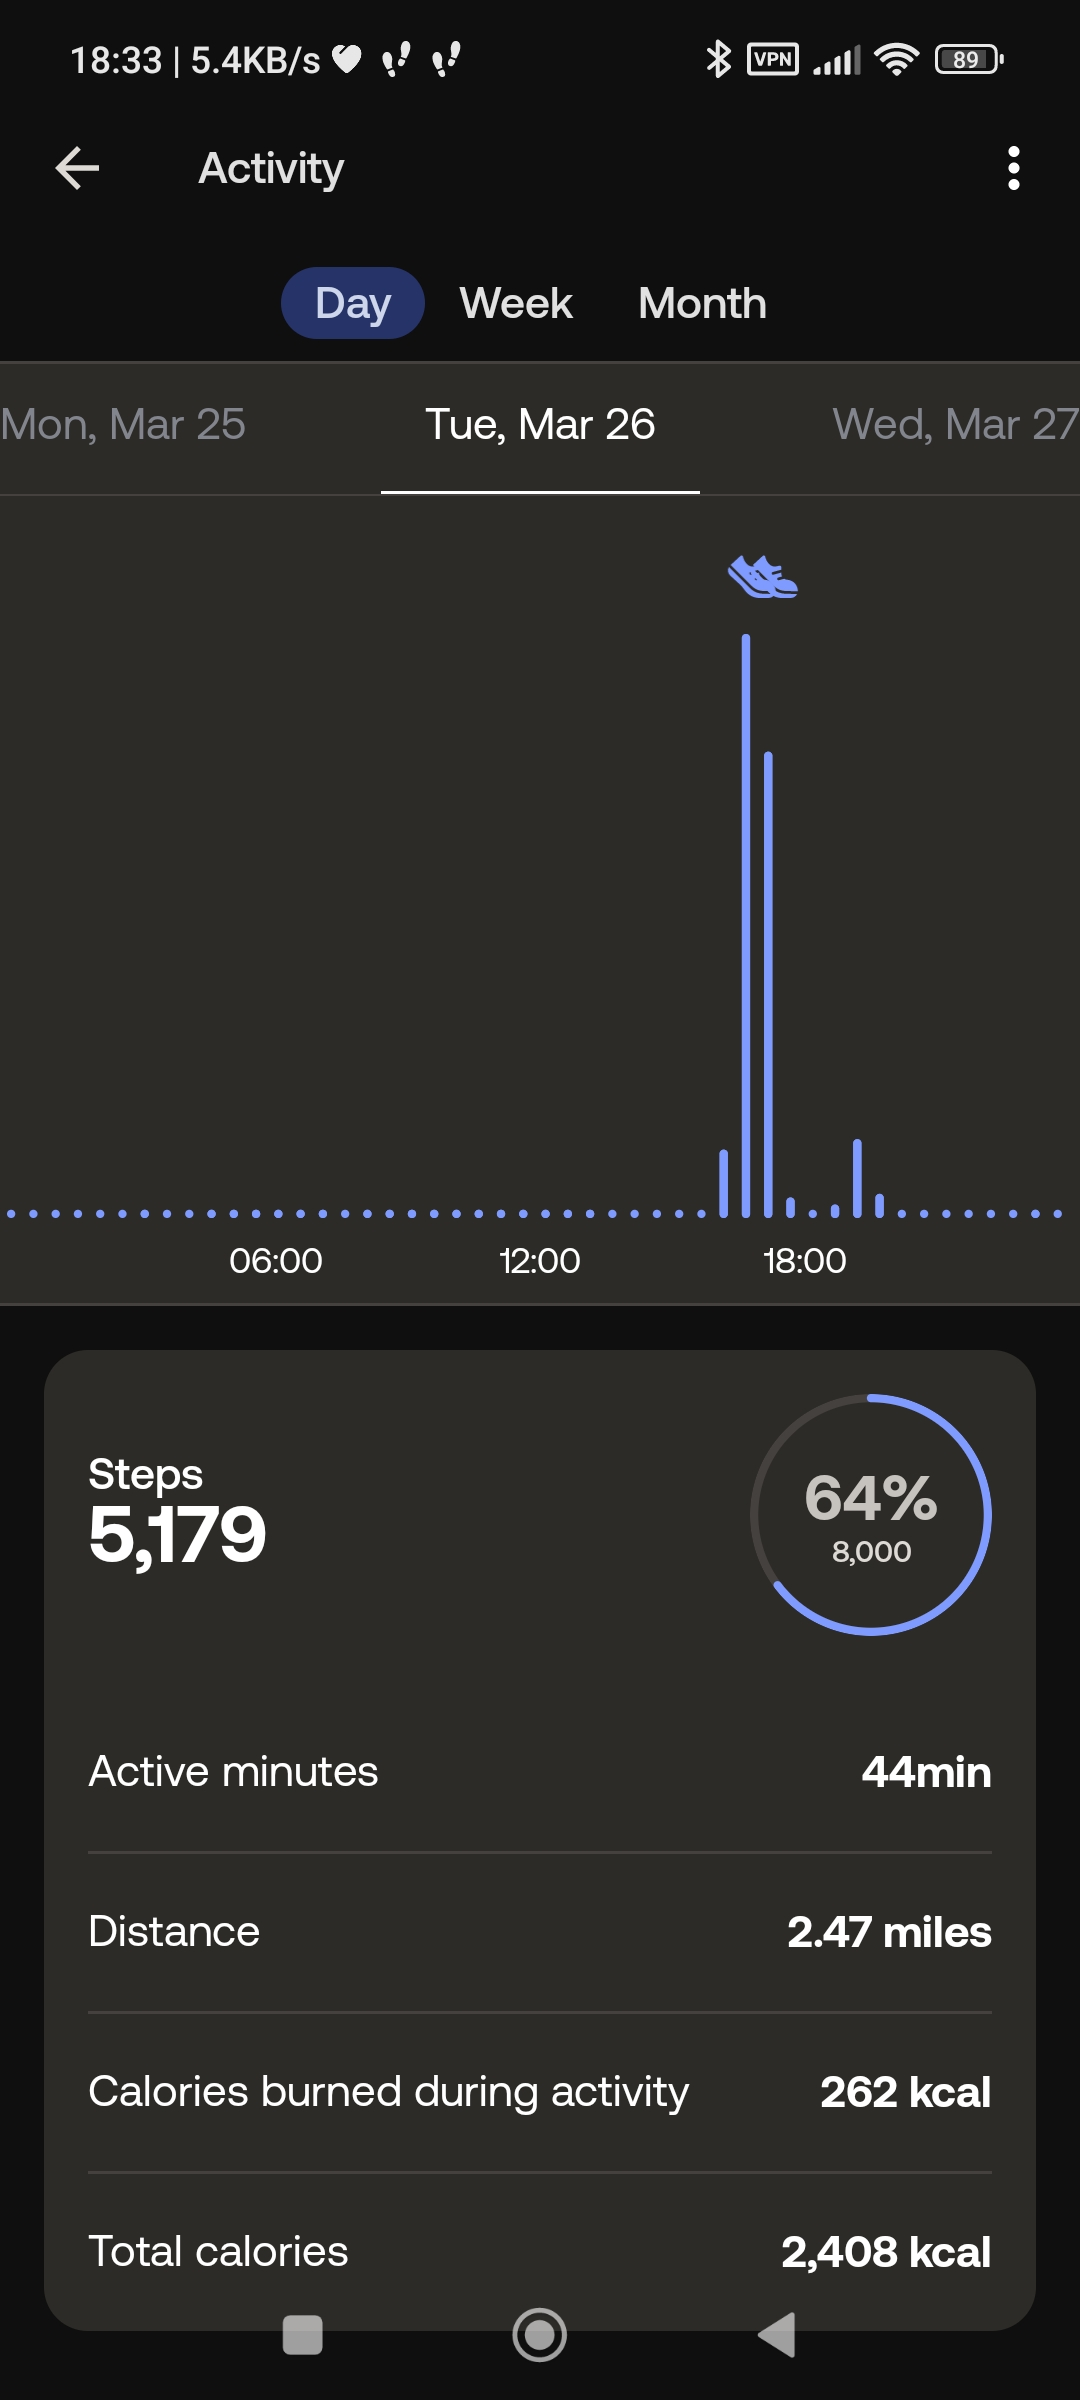
\includegraphics[width=0.5\textwidth,keepaspectratio]{../images/WithingsActivity.jpg}
    \caption{Withings Step count for 26th April}
    \label{fig:withingsSteps}
    
\end{figure}

\begin{figure}
    
    \centering
    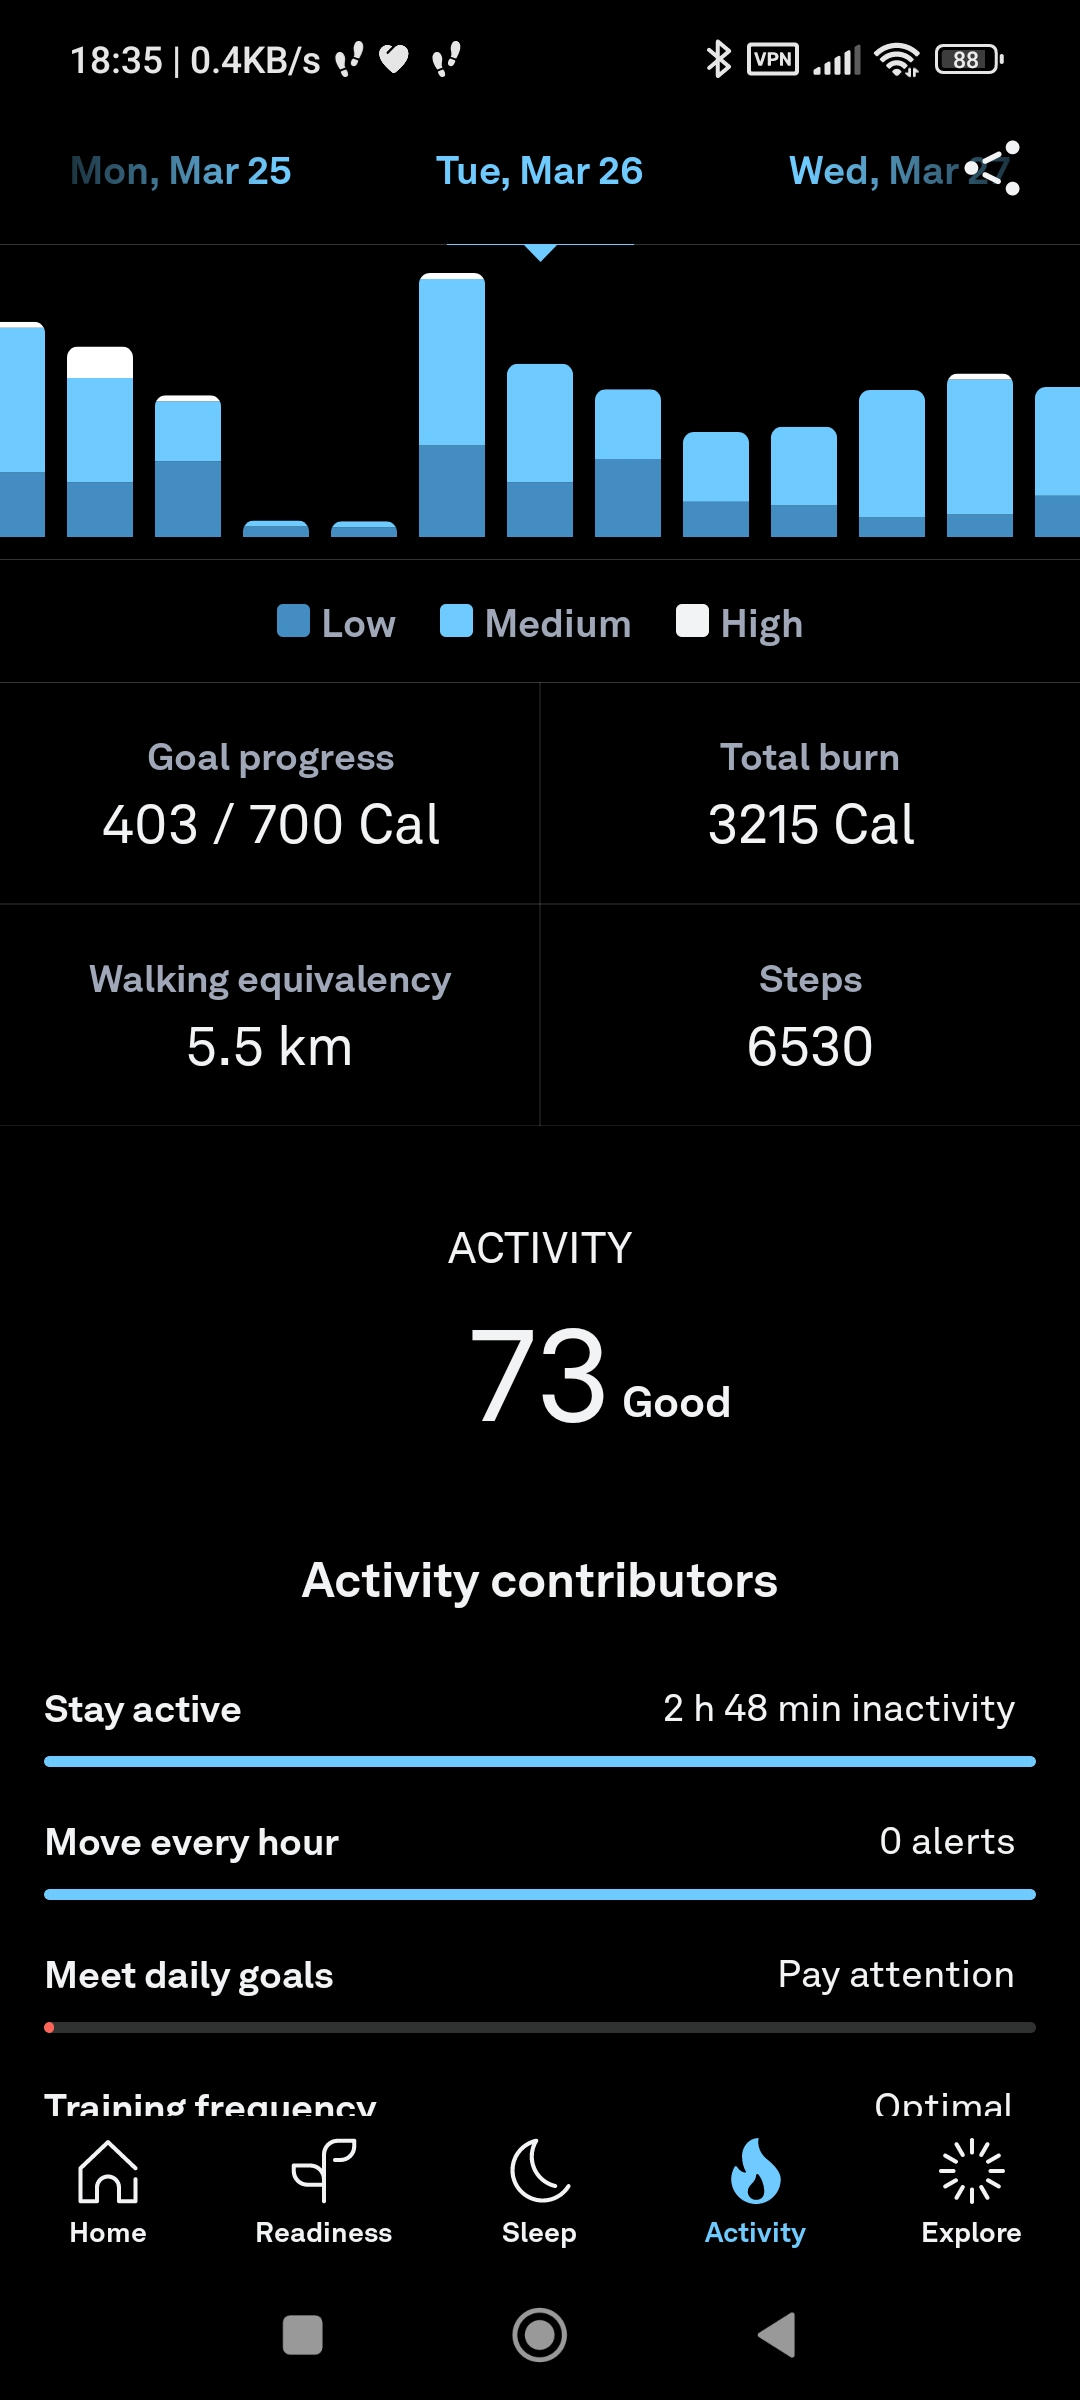
\includegraphics[width=0.5\textwidth,keepaspectratio]{../images/OuraActivity.jpg}
    \caption{Oura Step count for 26th April}
    \label{fig:ouraSteps}
    
\end{figure}
\begin{figure}
    
    \centering
    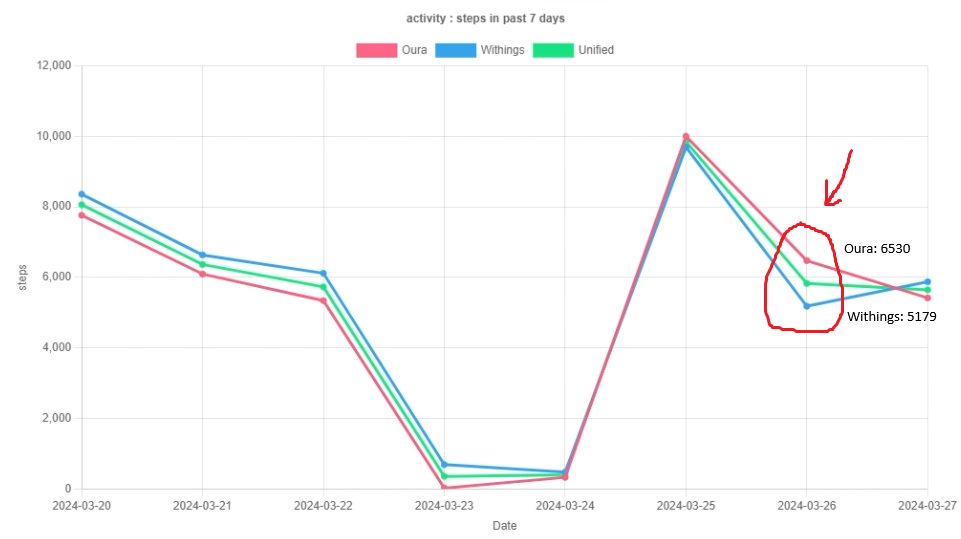
\includegraphics[width=0.9\textwidth,keepaspectratio]{../images/dashboard.png}
    \caption{OpenFitCompanion Step count for 26th April}
    \label{fig:openFitCompanionSteps}
    
\end{figure}
\section{Security}
\subsection{Automatic Vulnerability Scanners Testing}
Automatic web application vulnerability and penetration testing software was used to test security of the application. The following results were obtained: 
\begin{itemize}
    \item Wapiti (Open-source): \ref{fig:wapiti} (note: screenshot is trimmed, the rest of the report showed 0 vulnerabilities)
    \item ZAP (Open-source, made by OWASP): \ref{fig:zap}
    \item Intruder (Commercial, Large-scale grade): \ref{fig:intruder}
\end{itemize}
Scanners were used to probe how a person on the internet could try to breach the website - Scanners were not run in authenticated mode, since the authentication is only possible by the owner - since there is only one user, no privilege elevation vulnerability is possible. No critical or high risk vulnerabilities were discovered. ZAP gave false positives with hidden files, which in-fact are just like index.html for amplify, those don't expose any sensitive info.  Addressing interesting findings one by one: 
\begin{itemize}
    \item Clickjacking: this is an exploit when the website is embedded via iframe on attacker's website and original ui elements are masked behind fake ones. Although no information or access is exposed, attackers may force spending openAI credits by masking send prompt button. It kind of requires a targeted attack on the owner, which is a bit unlikely but the fix is an easy one line change, so it should have been implemented.
    \item Content-security policy (CSP): it is a primarily XSS mitigation, which in this application happens if the user willingly does it themselves or if providers get hacked and return XSS infected payloads. Although it is unlikely to happen, it is a quite easy fix and should have been implemented as well. 
    \item Strict Transport Security: Basically force HTTPS and don't allow HTTP. The default is HTTPS, and if the user purposefully goes to the HTTP version, it is mostly user error, however this may happen with less technical users. This was missed and should have been implemented
\end{itemize}
\begin{figure}
    
    \centering
    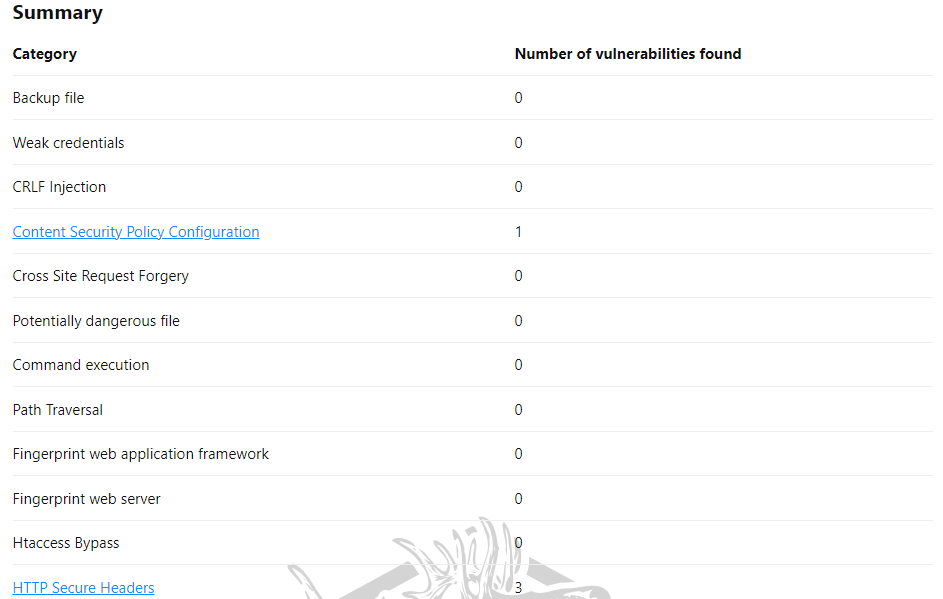
\includegraphics[width=0.9\textwidth,keepaspectratio]{../images/Wapiti.png}
    \caption{Wapiti scan result}
    \label{fig:wapiti}
    
\end{figure}
\begin{figure}
    
    \centering
    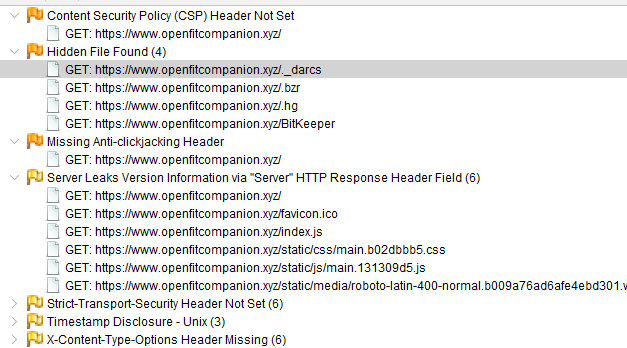
\includegraphics[width=0.8\textwidth,keepaspectratio]{../images/ZapResults.png}
    \caption{ZAP scan result}
    \label{fig:zap}
    
\end{figure}
\begin{figure}
    
    \centering
    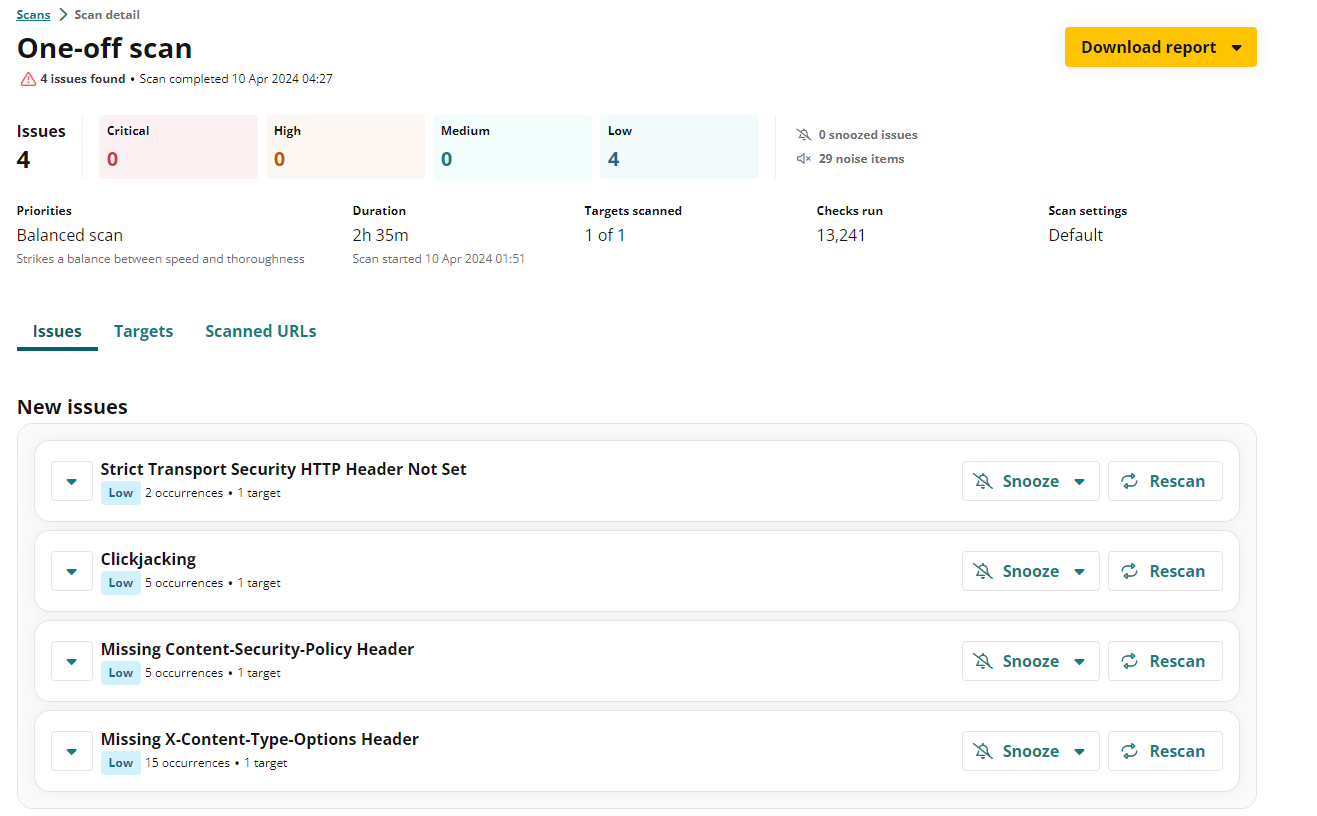
\includegraphics[width=1\textwidth,keepaspectratio]{../images/IntruderResults.png}
    \caption{Intruder scan result}
    \label{fig:intruder}
    
\end{figure}
\subsection{IAM}
AWS IAM access analyzer was used to find services that can be invoked externally: \ref{fig:awsexternal}. No issues were found, as those are the entrypoints to the system and no other service is exposed to the public. Note: test is a misnamed service for Withings notification handle and requestTokens is OAUTH callback handler for Withings as well.

Unfortunately, I was not able to find any AWS IAM role analyser for least privilege, so it was done manually: \ref{table:IAMroles}. All roles only had the minimal necessary permissions to perform their function. The system does not use virtual network so all functions can potentially make external requests - however, it should not be an issue, as external entities can't request into the network except for designated endpoints.
\begin{figure}
    
    \centering
    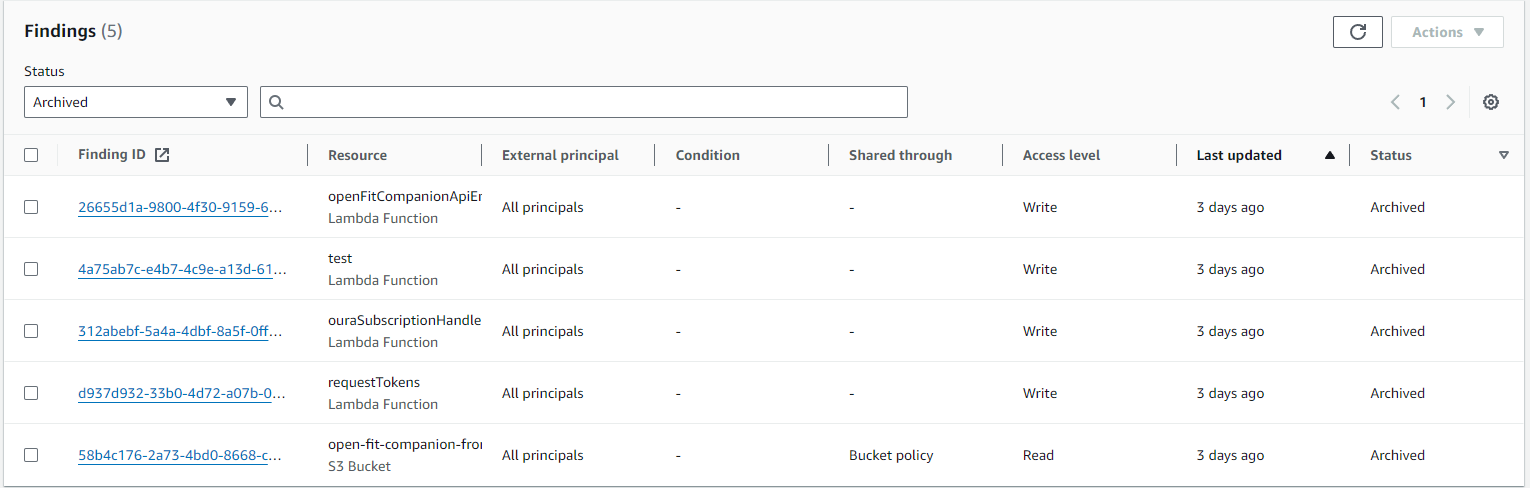
\includegraphics[width=1\textwidth,keepaspectratio]{../images/IAM_external.png}
    \caption{AWS Access analyzer - External access results}
    \label{fig:awsexternal}
    
\end{figure}
\begin{longtblr}[
    caption={IAM roles},
    label={table:IAMroles}
] {
    colspec = {|X|X|},
    rowhead = 1,
    hlines,
}
    Services & Permissions \\
    ApiEndpoint & DB: UserData: Read and Write; HealthData: Read; S3 exportBucket create object \\
    WithingsNotificationProcessor \& OuraNotificationProcessor & SNS publish \\
    ProcessNotification & DB: HealthData: Read and Write; Tokens: Read and Write; SQS: Read\\

\end{longtblr}
\section{Cost}

\subsection{Core Service}
Cost calculations were made using actual usage from February 2024, and pricing used is also from that period. Some services like cloudwatch (logging) or categories such as Amplify build artifacts, were used only for development and are not necessary to run the service, so they won't be in the list. Data export was done once. Table: \ref{table:awscost}
\begin{longtblr}[
    caption={AWS costs},
    label={table:awscost}
] {
    colspec = {|X|X|X|},
    rowhead = 1,
    hlines,
}
    Service & Usage & Cost \\
    Lambda & GB-seconds: 717 seconds; Requests: 4531 & 0.0129\$ \\
    DynamoDB & Read capacity unit hours: 2160; Write capacity unit hours: 2160; Storage: 182KB & 1.6848\$ \\
    Amplify & Data Out: 0.063GB & 0.00945\$ \\
    SNS & Requests: 810 & 0.000405\$ \\
    S3 & Storage: 0.003GB & 0.000069 \$ \\

\end{longtblr}
The total per month is: 1.7\$ or 1.29£. The only one that will increase with more usage is DynamoDB storage, however the health data is very light, with the entire table of 80 days weighing 120KB. AWS Always Free Tier covers all of the expenses for this typical usage, so actually 0£ are paid for the core application without AI. So, it can easily be used the same as aggregators like Google Fit or Apple Health, owning the data in your controlled infrastructure, without paying anything. However, it is worth to note that AWS can change any of the Free Tier reductions at any point, so minimising cost without it is still worth it.
\subsection{AI}
Using AI is where costs get more dire. At the time of writing, OpenAI charges 10\$ per 1M tokens with all GPT4 models, which is the one that is used. Due to the nature of RAG, the number of tokens used for a request varies, an average number of tokens is calculated from last 5 requests. Table: \ref{table:gptCosts} 
\begin{longtblr}[
    caption={GPT4 Costs},
    label={table:gptCosts}
] {
    colspec = {|X|X|X|},
    rowhead = 1,
    hlines,
}
    Prompt & Tokens & Cost \\
    Daily Feedback & 28643 tokens;  & 0.286\$ \\
    Activity Plan & 29566 tokens; & 0.295\$ \\
    Knowledge Retrieval & Files: 1;  & 0.2\$ \\
\end{longtblr}
So, the daily cost is 0.78\$ or 0.67£, translating to 20.15£ per month. That only accounts for automatic AI use, on-demand use through free-form chat would obviously increase this number. 
\subsection{Commercial product comparison}
Costs are compared to other commercially available products that provide guidance in health and/or fitness, although they offer quite different degrees of personalisation, with the ones that have AI in the name offering much closer experience to my product ideal - \ref{table:costCompare}.
\begin{longtblr}[
    caption={Cost Comparison},
    label={table:costCompare}
] {
    colspec = {|X|X|},
    rowhead = 1,
    hlines,
}
    Product & Monthly Cost \\
    OpenFitCompanion & 20.15£ (AI, rest Free Tier)  \\
    Apple Fitness+ & 9.99£ \\
    MyFitnessPal & 15.99£ \\
    EvolveAI & 19.99£ \\
    CoachifyAI & 28.49£ \\ 
    Withings+ & 8.95£

\end{longtblr}
Our product is not competitive with existing commercial products, only being cheaper than CoachifyAI. They would likely provide better quality insights due to having fine-tuned models and better rates with providers such as OpenAI, AWS, etc. In order to compete, our solution would need to be very cheap, like 7£ per month maximum, which the current solution fails at. I suspect that token counts are so bad because sometimes unnecessairy entries of health data are included, which we have no control of, as OpenAI says: "Retrieval currently optimizes for quality by adding all relevant content to the context of model calls. We plan to introduce other retrieval strategies to enable developers to choose a different tradeoff between retrieval quality and model usage cost." \cite{knowledgeRet}

\section{Customisability}
User requirements specified that all variables, configurations, etc should be easily customizable by a user, meaning it should be accessible to non-technical person, configuring through GUI. The following table summarises parameters in the system and whether they are fully customizable \ref{table:customizability}.
\begin{longtblr}[
    caption={Customizability of system},
    label={table:customizability}
] {
    colspec = {|X|X|},
    rowhead = 1,
    hlines,
}
    Parameter & Customisable? \\
    MET minutes target & Yes \\
    Home equipment & Yes \\
    Athleticism level & Yes \\
    Gym days & Yes \\
    Excluded activities & Yes \\
    Daily Report notification time & No \\
    Exercise notification time & No \\
    Concentration of exercises & No \\
    
\end{longtblr}
Scheduled events such as daily report notification as well as concentration of exercises (such as more exercises in the morning please) were hard-coded, as they would require a lot more work to implement. However, all else can be modified through GUI and that information is accurately reflected in insights.
\section{Frontend Performance \& Accessibility \& UI}
Lighthouse automated testing suite for web pages was used on every page, testing for mobile platform. However, SEO score was ignored, due to the nature of the application being a personal service rather than a public one. Screenshot of dashboard results \ref{fig:lighthouse}. Results are collated in a table: \ref{table:lighthouse}
\begin{longtblr}[
    caption={Lighthouse testing results},
    label={table:lighthouse}
] {
    colspec = {|X|X|X|X|},
    rowhead = 1,
    hlines,
}
    Page & Performance & Accessibility & Best Practices \\
    Dashboard & 93\% & 98\% & 96\% \\
    Daily Report & 92\% & 100\% & 96\% \\
    Weekly Report & 95\% & 100\& & 96\% \\
    Profile & 93\% & 100\% & 96\% \\
    Activity Plan (largest) & 82\% & 100\% & 96\% \\
    AI Chat & 94\% & 100\% & 96\% \\

\end{longtblr}
Performance results are satisfactory, ensuring snappy feel even when used on mobile network. No accessibility issues were found and best practices are strictly adhered to. Unfortunately all health data aggregators are app only, therefore it is not possible to directly compare their performance against ours; but for reference, sites with dynamic content in forms of graphs - such as Investing.com, have performance scores of around 60 (with adblock enabled). The score drops on Activity plan page, mainly due to exercise video examples via YouTube embeds, view only rendering may help to alleviate this, by only rendering components in the view. React lazy component loading should have been used to push the performance score a bit higher.
\begin{figure}
    
    \centering
    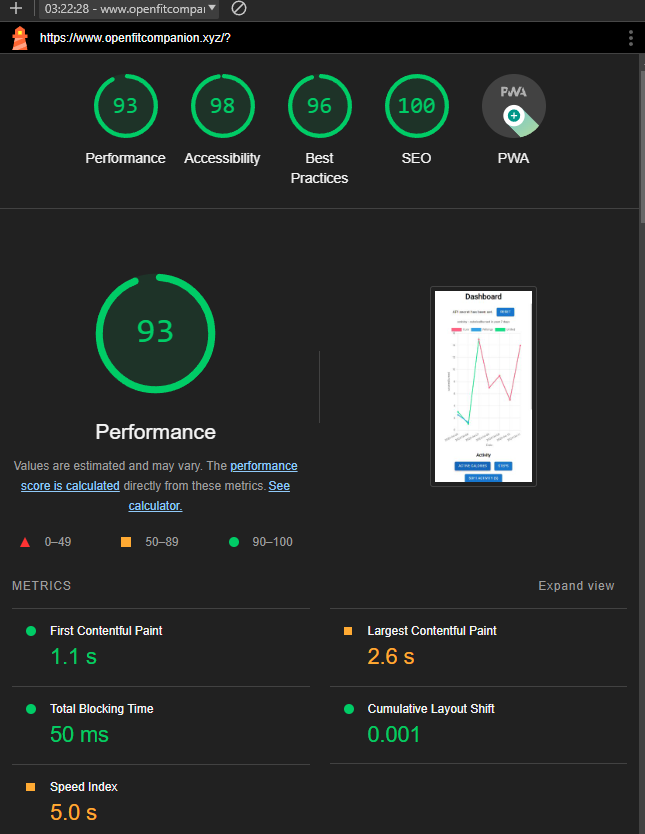
\includegraphics[width=1\textwidth,keepaspectratio]{../images/lightHouseMainPage.png}
    \caption{Lighthouse test result for dashboard}
    \label{fig:lighthouse}
    
\end{figure}

Each page has been evaluated for UI quality by checking if all applicable golden rules \ref{section:goldenRules} of UI are followed. For example, the profile page \ref{fig:profile} follows "Prevent errors" rule, as it uses proper input types, such as numeric only for weight field, preventing the user from entering invalid characters. However it does not follow: "Dialogs that yield closure", since no success message is displayed after form submission. Results are collated in the following table: \ref{table:goldenRulesUi}, with evaluation for each relevant rule having 3 possible values: "No", "Maybe", "Yes", with maybe used whenever it is up to the interpretation.
\begin{figure}
    
    \centering
    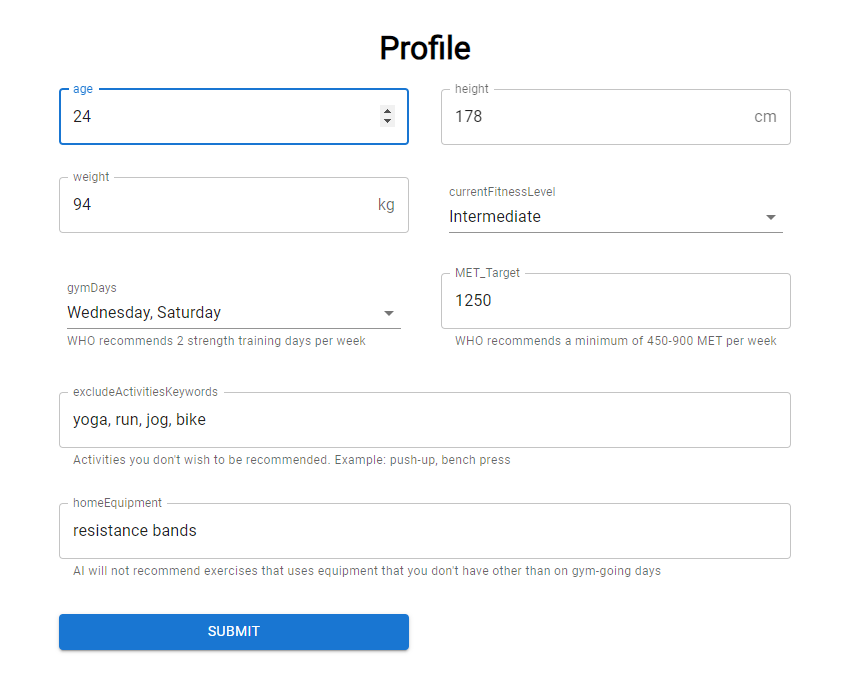
\includegraphics[width=1\textwidth,keepaspectratio]{../images/profilePage.png}
    \caption{Profile Page}
    \label{fig:profile}
    
\end{figure}
\begin{longtblr}[
    caption={Golden Rules UI evaluation results},
    label={table:goldenRulesUi}
] {
    colspec = {|X|X|},
    rowhead = 1,
    hlines,
}
    Page & Rules: Compliance \\
    Dashboard & 1: Yes; 2: Maybe; 3: Yes; 8: Yes \\
    Profile & 1: Yes; 2: Maybe; 3: Yes; 4: No; 5: Yes; 6: Yes; 8: Maybe \\
    Daily Report &  1: Yes, 2: Maybe, 8: Yes \\
    Weekly Report & 1: Yes, 2: Maybe, 8: Yes \\
    Exercise Plan & 1: Yes; 2: Maybe, 8: Maybe \\
    AI Chat & 1: Yes, 2: Maybe, 3: No, 4: No, 5: No, 6: No, 8: Yes \\

    
\end{longtblr}
To comment on a few interesting entries, universal usability compliance on any page is debatable, it can be used on any screen size and the language is quite simple to understand, however there are no internationalization such as other language versions or different date/calendar versions. AI chat was the worst performing one, as no feedback is displayed when user submits a prompt, only after manually refreshing the page the outcome is seen; also no reversal, no prevention of errors: users may put very long or complicated prompt that uses entire RAG file, which will burn through their OpenAI credits. 
\section{AI Insights Quality}
Providing quantifiable evidence of LLM response quality would be too complex and out of scope for this project. One good example and one bad example of an insight will be provided, as well as my qualitative thoughts about the insights after using the service as a normal user for 10 days. 
\begin{figure}
    
    \centering
    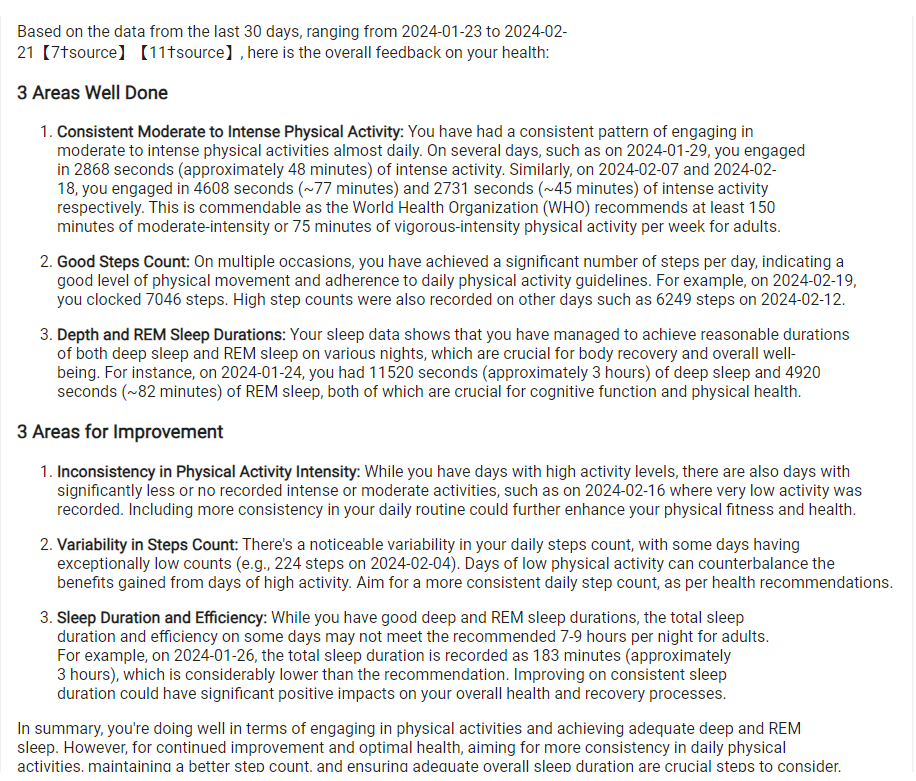
\includegraphics[width=1\textwidth,keepaspectratio]{../images/GoodAi.png}
    \caption{Good AI insight: Monthly feedback}
    \label{fig:goodAi}
    
\end{figure}
\begin{figure}
    
    \centering
    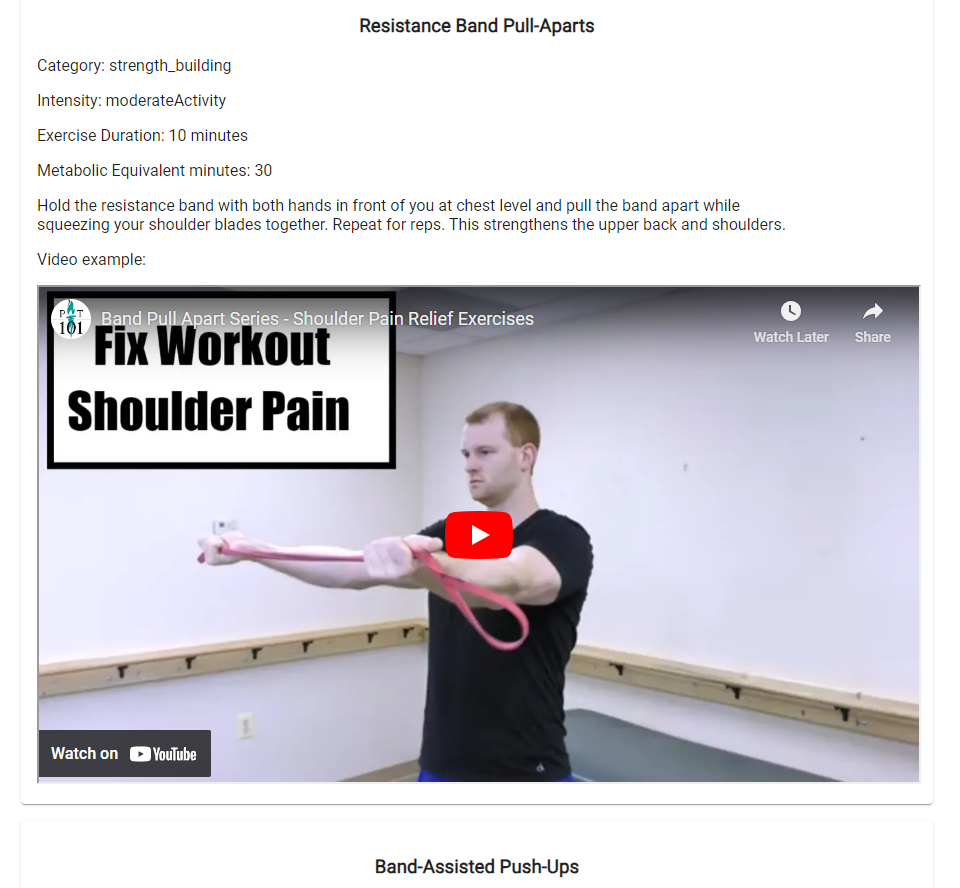
\includegraphics[width=1\textwidth,keepaspectratio]{../images/BadAi.png}
    \caption{Bad AI insight: Exercise Plan}
    \label{fig:badAi}
    
\end{figure}

One good thing I could point out, is LLM's ability to parse, analyse and spot some trend. A JSON file that is quite raw and unformatted for efficient analysis is uploaded and analysed successfully by GPT4. For example, when requesting a monthly feedback \ref{fig:goodAi}, it is able to point out variability in step count, showing on which day there were significantly less steps than in general trend. It was able to distinguish between variability/consistency versus mean, as it pointed that although mean physical activity per day is high, inconsistencies are also present, which is detrimental to the health. All of the findings I checked reflect reality, it does not invent numbers out of thin air, and insights are likely something that a human fitness coach would point out as well. 

One issue that I was not able to solve is "obsessiveness" towards some details. For example, on non-gym days exercises should have option to include using user's home equipment such as resistance bands. Unfortunately, after adding this to the instructions, nearly all exercises are to do with resistance bands \ref{fig:badAi}, which gets boring to the user. Nothing seemed to work to fix this, I've tried saying: "mix of home equipment exercises and no equipment needed exercises", "50\% home-equipment and 50\% no equipment needed", "prioritise variety of types of exercise", etc. It always came out on one side of the extreme, whereas the desired result is in the middle . 

Trends are often surface-level, with not much depth, they are mainly just picking out the obvious, which is something a normal person could do on their own anyway. For example, even on the good example \ref{fig:goodAi}, it picked out high steps counts and give a few examples. Another example was, when the daily feedback pointed that soft activity and steps were areas to be improved, however, they are very similar, so instead it could recommend to go on more walks to improve both metrics at the same time, rather than improving those metrics separately. Another negative point is that developing a good prompt requires a lot of trial-and-error, which is expected, but the price is charged per each attempt, I personally spent about 40£ on developing the prompts.
I think more work needs to be done to make insights more thorough and useful or the cost of inference has to go down, because currently ratio of utility to cost is low in my opinion.
\section{Comparing Devices - Discussing results}
Discussing \ref{fig:results}, to give an example of what equivalence bound is, at 95\% confidence, if we allow measurements to differ by more than 321 steps, then devices will be considered equal; consequently, any tolerance lower than that value will result in concluding that devices are different. It quantifies how much difference there is instead of just giving a binary answer of: reject null hypothesis of equivalence or not enough evidence. Both devices are equivalent in steps, even at 90\% confidence, which isn't included in the table for clarity. This is expected, as steps are not derived using bio data, but rather using dedicated hardware such as accelerometer, so the difference should not be large. I was not able to confirm it from the official documentation, but I suspect that the watch just classifies REM sleep as light sleep, since during the same time at night it shows REM sleep in the Oura app, while Withings has it as light sleep. This would essentially make sleep comparison not-valid, as they don't really measure the same metrics. The only sleep metric that is equivalent between devices is total sleep duration, although only at higher 99\% confidence. This reflects my personal experience, as the watch usually has a delay to detect that I am awake, around 10 minutes, so I would assume the same happens with falling asleep delay. It sums up to near 27 minutes difference, as calculated with the equivalence bound. This also suggests that devices might be similar for sleep tracking, but the comparison can't be made as the watch has a completely different framework with no REM sleep.  The one that is confusing is calories burned, which is deemed the same between two devices, but all other activity properties are significantly different, therefore it would make sense for calories to be different as well, as it is most likely derived from them. The watch tends to have more intense activity and the ring has more soft activity, so that overall difference balances out resulting in similar calories burned.

Answering the research question, there is evidence to suggest that devices might measure/classify activity metrics (soft, moderate, intense) differently. All of the other metrics either show equivalence or are not directly comparable. 